\documentclass[12pt]{article}

\usepackage[T1]{fontenc}
\usepackage{inconsolata}
\usepackage{xcolor}
\usepackage[utf8]{inputenc}
\usepackage{ngerman}
\usepackage{amsmath}
\usepackage{amssymb}
\usepackage{listings}
\usepackage{realboxes}
\usepackage{hyperref}
\usepackage{tikz}
\usepackage{float}
\usepackage{booktabs}
\usepackage{amsmath}

\definecolor{pblue}{rgb}{0.13,0.13,1}
\definecolor{pgreen}{rgb}{0,0.5,0}
\definecolor{pred}{rgb}{0.9,0,0}
\definecolor{pgrey}{rgb}{0.46,0.45,0.48}
\definecolor{mygray}{rgb}{0.9,0.9,0.9}

\lstset{language=Java,
  backgroundcolor=\color{mygray}
  showspaces=false,
  showtabs=false,
  breaklines=true,
  showstringspaces=false,
  breakatwhitespace=true,
  commentstyle=\color{pgreen},
  keywordstyle=\color{pblue},
  stringstyle=\color{pred},
  basicstyle=\ttfamily,
  moredelim=[il][\textcolor{pgrey}]{$$},
  moredelim=[is][\textcolor{pgrey}]{\%\%}{\%\%}
}

\newcommand{\type}[1]{<\negthickspace\text{#1}\negthickspace> }


\title{Code -- und Architekturanalyse}
\author{
        Klaus-Johan Ziegert\\
        MIN-Fakultät\\
        Fachbereich Informatik\\
        Studiengang: Informatik\\
        Matrikelnummer: 6523629\\
}
\date{\today}



\begin{document}
\maketitle
\begin{abstract}
        Diese Seminarausarbeitung dient der Vorbereitung des
        Masterprojektes ``Software-Engineering''. Das Ziel des
        Projektes ist die Entwicklung eines Werkzeuges, das die
        Analyse von bestehenden Softwaresystemen am Touchtisch
        und das Verstehen einer Software im Team ermöglicht. Um
        dieses Vorhaben zu verwirklichen, sind Kenntnisse von
        Code- und Architekturmetriken sowie die Untersuchung
        existierender Werkzeuge von Nöten, die in dieser
        Ausarbeitung vorgestellt werden.  Zum Schluss werden
        Anreize gegeben, welche umgesetzte Metriken von den Tools
        in das neue Werkzeug integriert werden sollten.
\end{abstract}

\newpage

\tableofcontents

\newpage

\section{Einleitung}
This is time for all good men to come to the aid of their party!

% \paragraph{Vorgehen}
% Im Kapitel \ref{metriken} wird die Definition, die Visualisierung
% als auch der allgemeine Umgang von Softwaremetriken beschrieben
% und erläutert. Daraufhin folgt im Kapitel \ref{codem} die
% Vorstellung von Codemetriken, eine detaillierte Beschreibung von
% CK-Metriken und die Untersuchung der CK-Metriken mit dem Tool
% ``geiler Tool'' an der Beispielsoftware ``verbesserungswürdige
% Software''.  Analog folgt Kapitel \ref{archm} mit den
% Archtiekturmetriken.  Als Vertreter von Archtiekturmetriken
% werden die weit bekannten Martins Metriken dienen und mit dem
% Tool ``geiler Tool'' am selbigen Beispielsoftware untersucht. Im
% vorletzten Kapitel \ref{tools} werden die unterschiedlichen Tools
% gegenübergestellt.  Der letzten Kapitel \ref{ausblick} dient als
% Ausblick für den zu entwerfenden Werkzeug, also wie und welche
% umgesetzte Metriken von den vorgestellten Tools in das neue
% Werkzeug integriert werden sollten.


\section{Softwaremetriken}\label{metriken}

\subsection{Definition und Ziele von Metriken}

Unter einer Softwaremetrik (abk. Metrik) versteht man eine
Funktion, die eine Eigenschaft von Software in einen Zahlenwert,
auch Maßzahl genannt, abbildet \cite{Wik18}. Die Eingabe einer Metrik ist
die Softwar-Einheit und die Ausgabe als Zahlenwert unterliegt
i.d.R. einer wohldefinierten Domäne. 
\\
\\
Abhängig von der untersuchten Software können folgende Arten von
Analysen vorgenommen werden:
\begin{itemize}
        \item statische Analyse durch den Quelltext
        \item dynamische Analyse beim Ausführen der
                kompilierten Datei
        \item historische Analyse durch Daten eines
                Versionskontrollsystem 
\end{itemize}
Diese Ausarbeitung beschränkt sich im Folgenden ausschließlich
auf die statische Analyse. Hiermit versteht man die Untersuchung
des jetztigen Ist-Zustand der Software. 
\\
\\
Es gibt eine Vielzahl von
Unterteilungen von Metriken, die Aussagen über den Ist-Zustand
treffen. Die wohl allgemeinste Unterteilung wird in \cite{Sne10} 
vorgeschlagen:

\begin{itemize}
        \item Quantität - Wie groß ist der Software-Einheit? Die
                Domäne ist die Menge der natürlichen Zahlen
                $\mathbb{N}$
        \item Qualität - Die Domäne ist..
        \item Komplexität - Wie umfangreich?
\end{itemize}
Zudem wird eine Metrik nicht auf das ganze Projekt angewendet.
Hierfür wird die hierachische Struktur des Software ausgenutzt,
d.h. man wendet die Metriken auf Packages, Klassen, Methoden usw.
an. So ordnet man die Untersuchung auf der Klassen- und
unterliegenden Softwarekomponenten-Ebenen der Codeanalyse, die
Untersuchung auf der Packages-Ebene der Archtiekturanalyse zu.
Wird eine Metrik hier angegeben, so wird der Name der Metrik
\textbf{metricname}, der Typ der Softwarekomponente $\type{type}$ und die
Domäne $D$ wie folgt spezifiziert:
\[
        \text{\textbf{metricname}}: ~ 
        \type{type}
        ~ \longrightarrow ~ D 
\]
Das übergeordnete Ziel der Untersuchung mithilfe von Metriken ist 
den Ist-Zustand mit einem Soll-Zustand zu vergleichen. Dabei
werden für die Metriken Schwellwerte definiert, die als
Indikatoren für sogenannte ''Bad-Smells'' dienen.

\subsection{Schwellenwerte}

Wenn der Wert einer Metrik durch eine Software-Einheit ermittelt
wird, so stellt man sich die Frage, ob dieser auf einen
schlechten Design hindeutet. Solch eine Entscheidung kann durch
Schwellenwerte entschieden werden, die lediglich als
Anhaltspunkte für einen Qualitätsmangel zu interpretieren sind.
Aufgrund des Mangels allgemeingültiger Schwellenwerte für
Metriken, ist es essentiell eigene Schwellenwerte zu ermitteln
oder den Hintergrund von empfohlene Schwellenwerte zu verstehen
und entsprechend anzupassen.
In \cite{Lan07} werden zwei Strategien zur Bestimmung von
Schwellenwerte präsentiert: statistische und ''sinnvolle''
Schwellenwerte.
\\
\\
\textbf{Statistische Schwellenwerte}. Man wählt eine Menge von
Software-Einheiten, die der zur untersuchenden Software-Einheit
am nächsten kommen (bspw. entschieden durch die Verwendung der selben
Programmiersprache), und berechnet für jede Metrik den
Durchschnitt AVG und die Standardabweichung STDEV. Hiermit können
folgende Schwellenwerte abgeschätzt werden:
\begin{itemize}
        \item Lower margin: AVG - STDEV
        \item Higher margin: AVG + STDEV
        \item Very high: (AVG + STDEV) $\cdot 1.5$
\end{itemize}
Liegt der Wert zwischen Higher margin und Very high, so sollte
die Software-Einheit genauer untersucht werden. Ist der Wert
jedoch höher als Very high, dann deutet dieser mit hoher
Wahrscheinlichkeit auf einen Qualitätsmangel hin.
\\
\\
\textbf{''Sinnvolle'' Schwellenwerte (engl. Meainingful
Thresholds)}.  Ist die Metrik auf 0 bis 1 normiert, so sind aus der
Statistik folgende Grenzen wohlbekannt:
\begin{itemize}
        \item 0.25 - One Quarter
        \item 0.33 - One Third 
        \item 0.5 - Half
        \item 0.66 - Two Thirds 
        \item 0.75 - Three Quarters 
\end{itemize}
Wenn ein Ausgleich (nahe 0.5) angestrebt wird, so können Werte
die Unterhalb von One Quarter oder Oberhalb von Three Quarters
mit hoher Wahrscheinlichkeit auf einen Qualitätsmangel hindeuten.
\\
\\
Ebenso können absolute Werte in ''sinnvolle'' Schwellenwerte
unterteilt werden. Der menschliche Kurzzeitgedächtnis kann etwa
bis zu 8 Elemente speichern und je geringer die Anzahl, desto
länger bleibt dies auch im Gedächtnis. Aus dieser Kenntnis können
folgende Schwellenwerte angegeben werden:
\begin{itemize}
        \item 0 - None
        \item 1 - One/Shallow
        \item 2--5 - Two, Three/Few/Several
        \item 7--8 - Short Memory Capacity
\end{itemize}
Der Umgang von Methoden mit mehr als 8 Zeilen kann bspw.
hierdurch als fraglich bestimmt werden.

\subsection{Visualisierung}

\subsection{DQM-Methode}

\section{Codemetriken}\label{codem}

\subsection{CK-Metriken}

\subsubsection{WMC}

Die erste CK-Metrik ist die Anzahl gewichteter Methoden
(engl. Weighted Method Count, abk. WMC). Diese Kenngröße
misst die Summe der Komplexitäten aller Methoden einer Klasse.
In \cite{chi94} wird die Bestimmung der Komplexität einer Methode
nicht festgelegt, so kann für die Komplexität einer Methode die
Anzahl der Codezeilen (LOC) oder die häufig mit WMC vorgestellte
Zyklomatische Komplexität nach McCabe (McCabe-Metrik) verwendet werden.
\[
        \text{WMC}: ~ 
        \type{class}
        ~ \longrightarrow ~ \mathbb{N}  \cup \left\{ 0 \right\} 
\]
Diese Metrik wird häufig als ein Maß für die Verständlichkeit und
Erweitbarkeit einer Klasse verstanden. Je mehr Methoden vorhanden
oder je komplexer die Methoden sind, desto größer sind die
Auswirkungen auf deren Unterklassen.

% \begin{figure}[H]
% \centering
%  \begin{tabular}{lcr}
%     \toprule
%     Good/Common & Regular/Casual & Bad/Uncommon \\
%     \midrule
%     $m \leq 11$ & $11 < m \leq 34$ & $m > 34$ \\
%     \bottomrule
%   \end{tabular}
%   \caption{Schwellenwerte für WMC aus \cite{Fil15}}
%   \label{tab:wmcthreshold}
% \end{figure}


\subsubsection{DIH}

Die zweite CK-Metrik ist die Tiefe der Vererbungshierarchie
(engl. Depth of Inheritance, abk. DIH). Diese Kenngröße misst die
Länge des maximalen Weges von der Wurzel bis zur betrachteten
Klasse im Vererbungsbaum. Der maximale Weg ist dann nur von
Interesse, wenn Mehrfachvererbungen möglich sind (bspw. C++).
\[
        \text{DIT}: \type{class} 
        \longrightarrow \mathbb{N} \cup \left\{ 0 \right\} 
\]
Diese Metrik wird häufig als Maß für die Testbarkeit und
Wartbarkeit verstanden. Je größer der Wert von DIH einer Klasse,
desto mehr Oberklassen gibt es und umso komplexer ist die Klasse.

% \begin{figure}[H]
% \centering
%  \begin{tabular}{lcr}
%     \toprule
%     Good/Common & Regular/Casual & Bad/Uncommon \\
%     \midrule
%     $m \leq 2$ & $2 < m \leq 4$ & $m > 4$ \\
%     \bottomrule
%   \end{tabular}
%   \caption{Schwellenwerte für DIT aus \cite{Fil15}}
%   \label{tab:ditthreshold}
% \end{figure}

\subsubsection{NOC}

Eine Ergänzung zu DIH ist die dritte CK-Metrik: die Anzahl der
Kinder in der Vererbungshierarchie (engl. Number of Children, abk.
Noc). Diese Kenngröße gibt für eine Klasse die Anzahl der
unmittelbaren abgeleitenden Klassen (auch Basisklassen) wieder.
\[
        \text{NOC}: \type{class} 
        \longrightarrow \mathbb{N} \cup \left\{ 0 \right\} 
\]
Ein hoher Wert von NOC bedeutet ein hohes Maß an
Wiederverwendung. Der Einflussbereich von Änderungen einer Klasse
mit hohem NOC kann hierbei bezüglich seiner Basisklassen steigen.
Solch eine Klasse erfordert wegen seiner zentralen Rolle
ebenfalls mehr Testaufwand.

% \begin{figure}[H]
% \centering
%  \begin{tabular}{lcr}
%     \toprule
%     Good/Common & Regular/Casual & Bad/Uncommon \\
%     \midrule
%     $m \leq 1$ & $1 < m \leq 3$ & $m > 3$ \\
%     \bottomrule
%   \end{tabular}
%   \caption{Schwellenwerte für NOC aus \cite{Fil15}}
%   \label{tab:nocthreshold}
% \end{figure}

\subsubsection{CBO}

Die vierte Metrik einer Klasse ist die Anzahl der gekoppelten
Klassen (engl. Coupling between Objects, abk. CBO). Eine Klasse A
ist mit einer anderen Klasse B genau dann gekoppelt, wenn A über
eine Referenz Zugriff auf B oder umgekehrt hat.
\[
        \text{CBO}: \type{class}
        \longrightarrow \mathbb{N} \cup \left\{ 0 \right\} 
\]
CBO ist ein Maß für die Wiederverwendbarkeit und Testbarkeit. Je
höher die Kopplung ist, desto schwieriger versteht man die Klasse,
sodass Verwendung und Tests eher dazu geneigt sind geringer auszufallen. 


% \begin{figure}[H]
% \centering
%  \begin{tabular}{lcr}
%     \toprule
%     Good/Common & Regular/Casual & Bad/Uncommon \\
%     \midrule
%     $m \leq <++>$ & $<++> < m \leq <++>$ & $m > <++>$ \\
%     \bottomrule
%   \end{tabular}
%   \caption{Schwellenwerte für CBO aus \cite{Fil15}}
%   \label{tab:cbothreshold}
% \end{figure}

\subsubsection{RFC}

Die fünfte CK-Metrik ist die Anzahl potenzieller Zielmethoden (engl. Response
for Class, abk. RFC). Diese Kenngröße misst die Anzahl aller
ausführbaren Methoden einer Klasse. Zu den definierten Methoden
der Klasse werden ebenfalls die von der Instanz anderer Klassen
aufgerufenen Methoden innerhalb der Klasse mitgezählt.
\[
        \text{RFC}: \type{class}
        \longrightarrow \mathbb{N} \cup \left\{ 0 \right\} 
\]
RFC gibt eine obere Schranke für die Anzahl der Testfälle an, die
durch die möglichen Methodenaufrufen notwendig werden.

% \begin{figure}[H]
% \centering
%  \begin{tabular}{lcr}
%     \toprule
%     Good/Common & Regular/Casual & Bad/Uncommon \\
%     \midrule
%     $m \leq <++>$ & $<++> < m \leq <++>$ & $m > <++>$ \\
%     \bottomrule
%   \end{tabular}
%   \caption{Schwellenwerte für RFC aus \cite{Fil15}}
%   \label{tab:rfcthreshold}
% \end{figure}



\subsubsection{LCOM}

Die letzte hier vorgestellte CK-Metrik ist 
der Zusammenhalt der Methoden (engl. Lack of cohesion in methods, abk. LCOM).
Diese Kenngröße misst die Anzahl aller möglichen
Methodenpaare, die keine Instanzvariable gemeinsam haben,
subtrahiert mit der Anzahl aller Methodenpaare, die mindestens
eine Instanzvariable gemeinsam haben. Falls der Wert von LCOM
negativ sein sollte, wird für LCOM 0 angenommen. 

% % \begin{figure}[H]
% % \centering
% %  \begin{tabular}{lcr}
% %     \toprule
% %     Good/Common & Regular/Casual & Bad/Uncommon \\
% %     \midrule
% %     $m \leq 0.167$ & $0.167 < m \leq 0.725$ & $m > 0.725$ \\
% %     \bottomrule
% %   \end{tabular}
% %   \caption{Schwellenwerte für LCOM aus \cite{Fil15}}
% %   \label{tab:lcomthreshold}
% % \end{figure}
% %

LCOM gibt den Grad der Kapselung der Methoden wieder. Je größer
der Wert von LCOM ist, desto weniger haben die Methoden
miteinander zu tun.

\subsection{``geiler Tool'' und Bewertung}

\section{Archtiekturmetriken}\label{archm}

\subsection{Martins Metriken}

\subsubsection{CA}\label{CA}

Die erste Martin-Metrik ist die afferente Kopplung (eng. afferent
Coupling, abk. CA, in \cite{Sne10} eine Kenngröße).
Diese Kenngröße misst für ein Package $P$ die Anzahl der Packages,
die von Klassen innerhalb von $P$ abhängen. Man spricht daher von
der Anzahl der eingehenden Abhängigkeiten.
% Die eingehenden Abhängigkeiten werden in einem Java-Quelltext mit
% der Anweisung \lstinline|import P.*| außerhalb des zu
% untersuchenden Packages ermittelt.
\[
        \text{CA}: \textless \text{Package} \textgreater
        \longrightarrow \mathbb{N} \cup \left\{ 0 \right\} 
\]
Das Modifizieren eines Packages $P$ mit eingehenden
Abhängigkeiten führt i.d.R. zu weitreichenden Anpassungen der
zugehörigen Packages. Der Arbeitsaufwand wächst daher mit der Größe von
CA, sodass generell Modifikationen eines Packages mit hohen CA
gemieden werden soll.  Ein hoher Wert von CA deutet demnach auf
eine hohe Stabilität hin.

% \begin{figure}[H]
% \centering
%  \begin{tabular}{lcr}
%     \toprule
%     Good/Common & Regular/Casual & Bad/Uncommon \\
%     \midrule
%     $m \leq 7$ & $7 < m \leq 39$ & $m > 39$ \\
%     \bottomrule
%   \end{tabular}
%   \caption{Schwellenwerte für CA aus \cite{Fil15}}
%   \label{tab:cathreshold}
% \end{figure}

\subsubsection{CE}\label{CE}

Die zweite Martin-Metrik ist die efferente Kopplung (engl.
efferent Coupling, abk. CE, in \cite{Sne10} eine Kenngröße).
Diese Kenngröße ist das Gegenstück zu CA, denn sie misst für ein
Package $P$ die Anzahl der Packages, von denen Klassen innerhalb
von $P$ abhängen. Man spricht daher von der Anzahl der
ausgehenden Abhängigkeiten.
% Die ausgehenden Abhängigkeiten
% werden in einem Java-Quelltext mit der Anweisung
% \lstinline|import notP| innerhalb des zu untersuchenden Packages
% ermittelt.
\[
        \text{CE}: \textless \text{Package} \textgreater \longrightarrow \mathbb{N} \cup 0
\]
Wenn ein ausgehend abhängiges Package $P_{out}$ modifziert wird,
so muss i.d.R. das Package $P$ entsprechend der Modifikationen
von $P_{out}$ angepasst werden. Die Häufigkeit solcher
Modifkationen steigt daher tendentiell mit dem Wert
von CE. Ein hoher Wert von CE deutet demnach auf eine hohe
Instabiltät hin.

% \begin{figure}[H]
% \centering
%  \begin{tabular}{lcr}
%     \toprule
%     Good/Common & Regular/Casual & Bad/Uncommon \\
%     \midrule
%     $m \leq 6$ & $6 < m \leq 16$ & $m > 16$ \\
%     \bottomrule
%   \end{tabular}
%   \caption{Schwellenwerte für CE aus \cite{Fil15}}
%   \label{tab:cethreshold}
% \end{figure}

\subsubsection{I}\label{I}

Die dritte Martin-Metrik ist die Instabilität (eng. Instability, abk.
I). Diese Metrik liefert das Verhältnis der Anzahl der
ausgehenden Abhängigkeiten zu der Anzahl aller
Abhängigkeiten, also:
\[
        I = \frac{CE}{CE + CA}
\]
mit
\[
        \text{I}: \textless \text{Package} \textgreater
        \longrightarrow [0,1] \subset \mathbb{R}
\]
Ein hoher Wert von $I$ (nah bei 1) bedeutet, dass das Package
überwiegend mehr ausgehende Abhängigkeiten besitzt. Es finden
dann häufiger Anpassungen an solch einem Package statt, jedoch ist
der Arbeitsaufwand generell gering.  Ein geringer Wert von $I$
(nah bei 0) bedeutet, dass das Package überwiegend mehr
eingehenden Abhängigkeiten besitzt. Der Arbeitsaufwand ist
relativ groß, hierfür treten Anpassungen generell selten auf. Als
Problematisch wird ein ausbalancierter Wert von CE (nah bei 0.5)
angesehen. Der relativ häufige und relativ große Arbeitsaufwand deuten
auf ein schlechten Softwaredesign hin.

% \begin{figure}[H]
% \centering
%  \begin{tabular}{lcr}
%     \toprule
%     Good/Common & Regular/Casual & Bad/Uncommon \\
%     \midrule
%     $m \leq <++>$ & $<++> < m \leq <++>$ & $m > <++>$ \\
%     \bottomrule
%   \end{tabular}
%   \caption{Schwellenwerte für I aus \cite{Fil15}}
%   \label{tab:ithreshold}
% \end{figure}

% \subsubsection{Konkrete Klassen (CC)}
% Die vierte Martin-Metrik ist die Anzahl der konkreten Klassen
% eines Packages (engl. Concrete Classes, abk. CC, in
% \cite{Sne10} eine Kenngröße). 
%
% \subsubsection{Abstrakte Klassen (AC)}

\subsubsection{A}

Die vierte Martin-Metrik ist die Abstraktion (engl. Abstractness,
abk. A) Diese Metrik gibt das Verhältnis der Anzahl der
abstrakten Klassen (engl. Abstract Classes, abk. AC, in
\cite{Sne10} eine Kenngröße) zu der Anzahl aller Klassen, also
abstrakten und konkreten Klassen (engl.  Concrete Classes, abk
CC, in \cite{Sne10} eine Kenngröße), wieder. Dabei zählt man zu
den abstrakten Klassen ebenfalls die Interfaces hinzu.
% Die
% Anzahl der abstrakten Klassen werden in einem Java-Quelltext mit
% den Schlüsselwörter \lstinline|abstract| und
% \lstinline|interface| innerhalb des zu untersuchenden Packages
% ermittelt. Die konkreten Klassen werden entsprechend durch
% die Abwesenheit dieser Schlüsselwörter gewonnen.
\[
        A = \frac{AC}{AC + CC}
\]
mit
\[
        \text{A}: \textless \text{Package} \textgreater
        \longrightarrow [0,1] \subset \mathbb{R}
\]
Ein hoher Wert von A (nahe 1) bedeutet, dass im Verhältnis sehr
viele abstrakten Klassen enthalten sind. Hierdurch werden
Erweiterungen begünstigt.  Ein niedriger Wert von A (nahe 0)
bedeutet analog überwiegend mehr konkrete Klassen. Modifkationen
sollen dann nach \cite{Mar94} deutlich einfacher fallen. 

% \begin{figure}[H]
% \centering
%  \begin{tabular}{lcr}
%     \toprule
%     Good/Common & Regular/Casual & Bad/Uncommon \\
%     \midrule
%     $m \leq <++>$ & $<++> < m \leq <++>$ & $m > <++>$ \\
%     \bottomrule
%   \end{tabular}
%   \caption{Schwellenwerte für A aus \cite{Fil15}}
%   \label{tab:athreshold}
% \end{figure}
\subsubsection{D}

Die letzte hier vorgestellte Martin-Metrik ist die normalisierte
Distanz von der Hauptsequenz (engl. Normalized Distance From Main
Sequence, abk. D). Diese Metrik gibt die Balance der Abstraktion
A und Instabilität I wieder.
\[
        D = |A + I - 1|
\]
mit 
\[
        \text{D}: \textless \text{Package} \textgreater
        \longrightarrow [0,1] \subset \mathbb{R}
\]
In der Darstellung \ref{fig:ai-graph} ist der sogenannte AI-Graph
mit der Instabilität an der horizontalen und der Abstraktion an
der vertikalen Achse angegeben \cite{Mar94}.  Nach \cite{Mar94}
gibt es für ein Package zwei anzustrebende AI-Tupel. Entweder das
Package ist stabil und abstrakt (nahe zu (0,1), der linke rote
Punkt) oder das Package ist instabil und konkret (nahe zu (1,0),
der rechte rote Punkt). Ebenso gibt es zwei zu meidende AI-Tupel,
nämlich ein abstraktes und stabiles Package (nahe zu (0,0), der
blaue Punkt) oder ein konkretes und instabiles Package (nahe zu
(1,1); der grüne Punkt). AI-Tupel eines Packages, die sich eher dem blauen Punkt
nähern, befinden sich im sogenannten ''Schmerzbereich''.
Zugehörige Packages sind kaum erweiterbar, werden jedoch häufig
von andere Packages genutzt. AI-Tupel eines Packages, die sich eher dem grünen Punkt
nähern, befinden sich im Bereich der sogenannten Nutzlosigkeit.
Solche Packages werden kaum genutzt, obwohl der Abstraktionsgrad
dies begünstigt. Aufgrund der anzustrebende Nähe der roten Punkte
und der anzustrebende Distanz der anderen Punkten hat sich die
Hauptsequenz als bevorzugtes Gleichgewicht ergeben; in der
Abbildung durch eine von beiden roten Punkte verbundene Linie
dargestellt. Die Metrik D gibt hierbei die absolute Distanz des
AI-Tupels zu der Hauptsequenz an.

% \begin{figure}[H]
% \centering
%  \begin{tabular}{lcr}
%     \toprule
%     Good/Common & Regular/Casual & Bad/Uncommon \\
%     \midrule
%     $m \leq <++>$ & $<++> < m \leq <++>$ & $m > <++>$ \\
%     \bottomrule
%   \end{tabular}
%   \caption{Schwellenwerte für D aus \cite{Fil15}}
%   \label{tab:dthreshold}
% \end{figure}


\begin{figure}[H]
        \centering
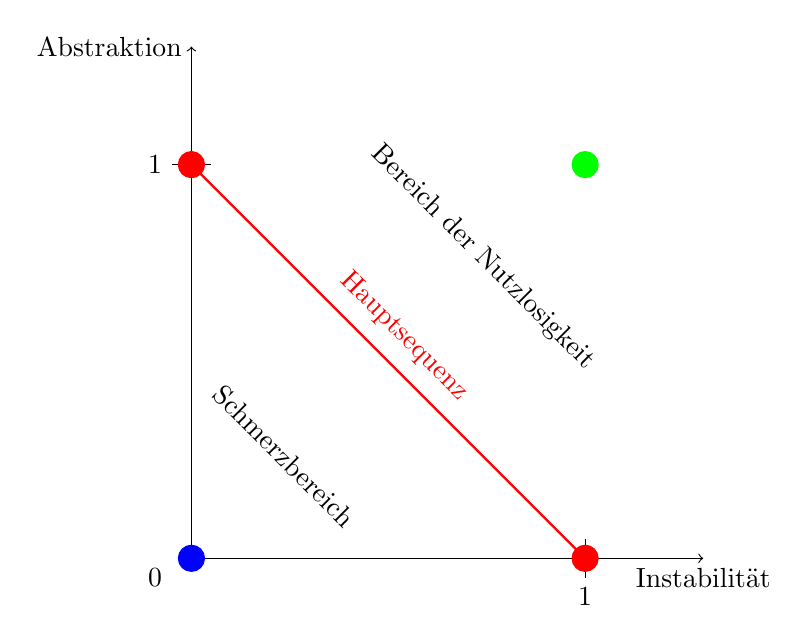
\begin{tikzpicture}[xscale=5,yscale=5,domain=0:1,samples=50]
    \draw[->] (0,0) -- (1.3,0) node[below] {Instabilität};
    \draw[->] (0,0) -- (0,1.3) node[left] {Abstraktion};
    \draw (0.05,1) --  (-0.05,1) node[left] {$1$}; 
    \draw (1,0.05) --  (1,-0.05) node[below] {$1$}; 
    \draw[red,thick] plot (\x,{1-\x});
    \node[label={[red, rotate=-45] Hauptsequenz}] at (0.5,0.5) {};
    \node[label={[rotate=-45] Schmerzbereich}] at (0.2,0.2) {};
    \node[label={[rotate=-45] Bereich der Nutzlosigkeit}] at (0.7,0.7) {};
    \node[below,left] at (-0.05,-0.05) {0};
    \node[draw,green,shape=circle,fill] at (1,1) {};
    \node[draw,blue,shape=circle,fill] at (0,0) {};
    \node[draw,red,shape=circle,fill] at (1,0) {};
    \node[draw,red,shape=circle,fill] at (0,1) {};
\end{tikzpicture}
\caption{AI-Graph \cite{Mar94}}
\label{fig:ai-graph}
\end{figure}




\subsection{``geiler Tools'' und Bewertung}

\section{Tools}\label{tools}

\section{Ausblick}\label{ausblick}

\newpage

\bibliographystyle{alphadin}
\bibliography{../Literatur/lit}{}

\end{document}
